\section{Results}
\label{sec:exp-results}


\begin{figure*}[ht]
\centering
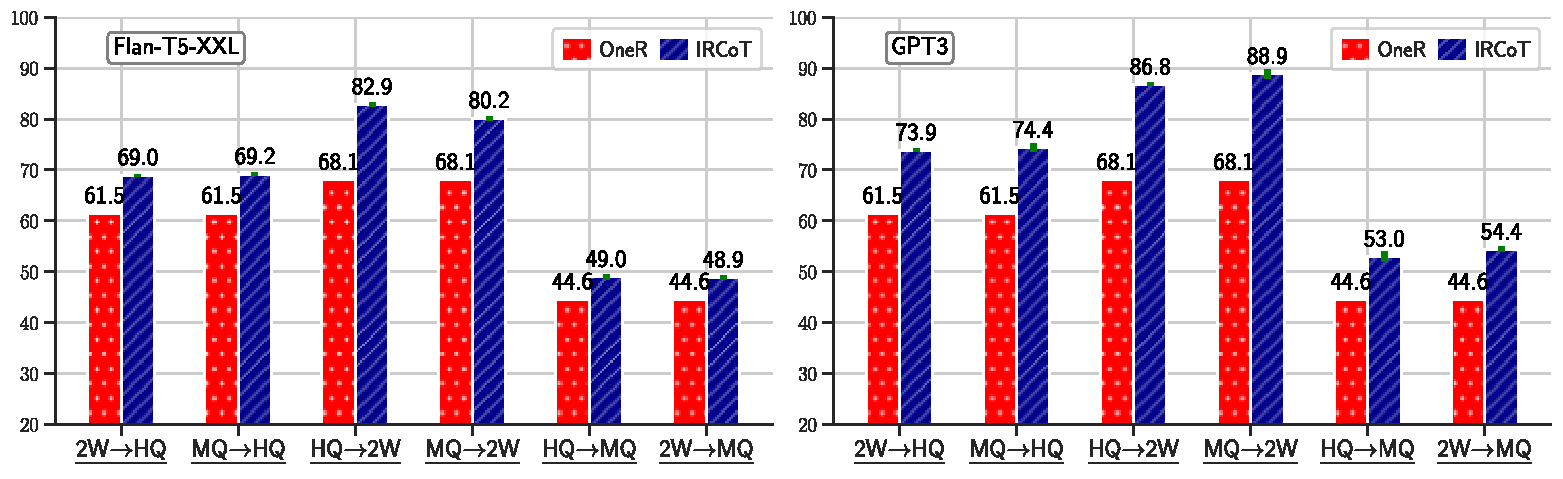
\includegraphics[width=0.95\textwidth]{images/ood_retrieval_results.pdf}
\caption{Retrieval recall for OneR and IRCoT using Flan-T5-XXL (Left) and GPT3 (Right) in out-of-distribution (OOD) setting. HQ (HotpotQA), 2W (2WikiMultihopQA), MQ (MuSiQue). The result X$\rightarrow$Y indicates prompt demonstrations are from dataset X and evaluation is on dataset Y. \iconsys outperforms OneR in such an OOD setting.}
\label{fig:ood-retrieval-results}
\end{figure*}

\begin{figure*}[ht]
\centering
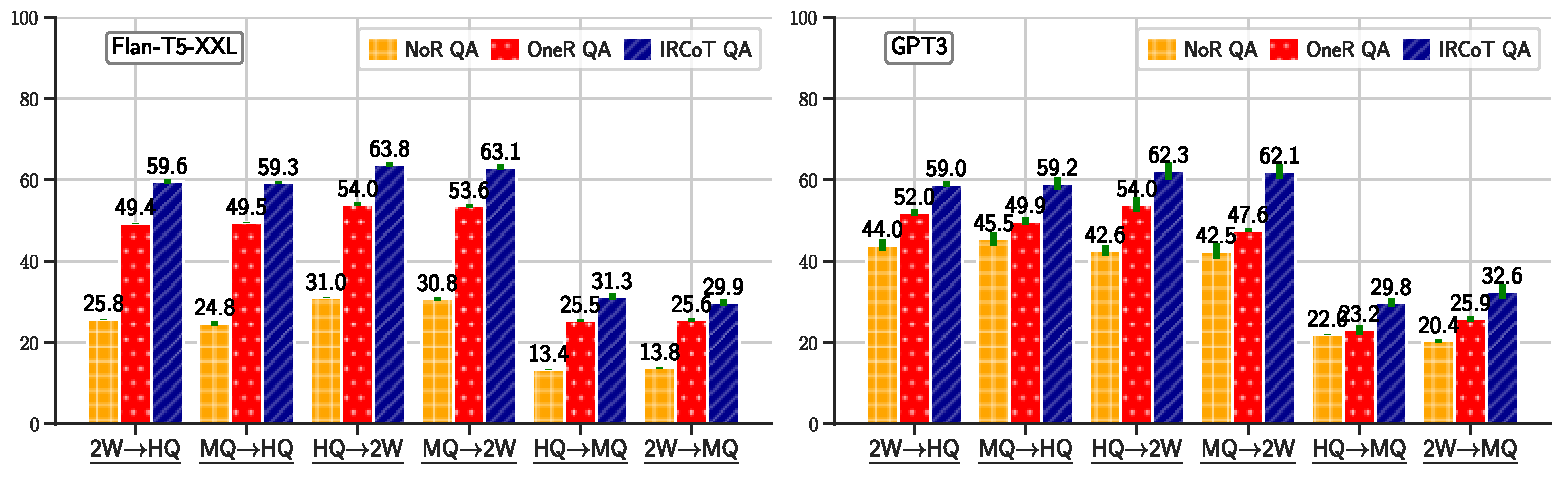
\includegraphics[width=0.95\textwidth]{images/ood_qa_results.pdf}
\caption{Answer F1 for NoR QA, OneR QA and IRCoT QA using Flan-T5-XXL (Left) and GPT3 (Right) in out-of-distribution (OOD) setting. HQ (HotpotQA), 2W (2WikiMultihopQA), MQ (MuSiQue). The result X$\rightarrow$Y indicates prompt demonstrations are from dataset X and evaluation is on dataset Y. \iconsys QA outperforms OneR QA and NoR QA in such OOD setting.}
\label{fig:ood-qa-results}
\end{figure*}


%%%%%%%%%%%%%%%%%%%%%%%%%%%%%%%%%%%%%%%%%%%%%%%%%%%%
\paragraph{\iconsys retrieval is better than one-step. }

Fig.~\ref{fig:main-retrieval-results} compares OneR with \iconsys retrievers made from \texttt{Flan-T5-XXL} and \texttt{GPT3} LMs. For both models, \iconsys significantly outperforms one-step retrieval across all datasets. For \texttt{Flan-T5-XXL}, \iconsys improves our recall metric relative to one-step retrieval, on HotpotQA by 7.9, on 2WikiMultihopQA by 14.3, on MuSiQue by 3.5, and on IIRC by 10.2 points. For \texttt{GPT3}, this improvement is by 11.3, 22.6, 12.5, and 21.2 points, respectively.

%%%%%%%%%%%%%%%%%%%%%%%%%%%%%%%%%%%%%%%%%%%%%%%%%%%%
\paragraph{\iconsys QA outperforms NoR and OneR QA.}

Fig.~\ref{fig:main-qa-results} compares ODQA performance using NoR, OneR and \iconsys retriever made from \texttt{Flan-T5-XXL} and \texttt{GPT3} LMs. For \texttt{Flan-T5-XXL}, \iconsys QA outperforms OneR QA on HotpotQA by 9.4, on 2WikiMultihopQA by 15.3, on MuSiQue by 5.0 and IIRC by 2.5 F1 points. For \texttt{GPT3}, the corresponding numbers (except for IIRC) are 7.1, 13.2, and 7.1 F1 points. For \texttt{GPT3}, \iconsys doesn't improve the QA score on IIRC, despite significantly improved retrieval (21 points as shown in Fig.~\ref{fig:main-retrieval-results}). This is likely because IIRC relevant knowledge may already be present in GPT3, as also evidenced by its NoR QA score being similar. For other datasets and model combinations, NoR QA is much worse than \iconsys QA, indicating the limits of the models' parametric knowledge.


\begin{figure}[ht]
\centering
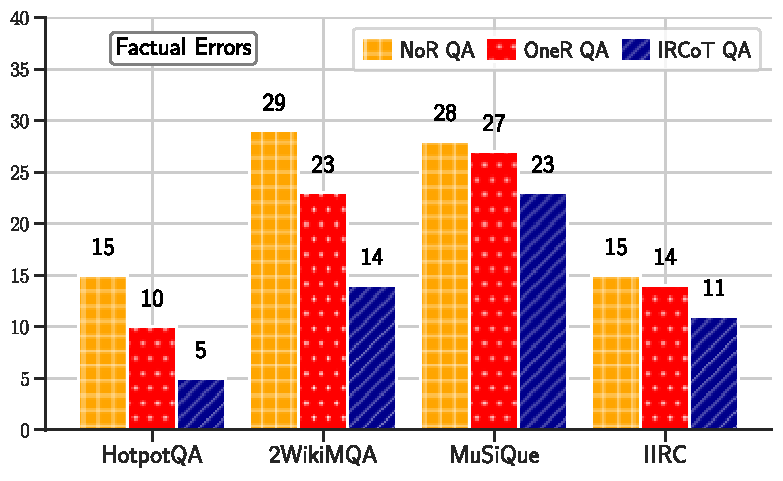
\includegraphics[width=0.475\textwidth]{images/factual_errors.pdf}
\caption{Number of questions, out of 40, where CoT generated by GPT3 using different methods has at least 1 factual error. Factual errors: \iconsys $<$ OneR $<$ NoR.}
\label{fig:cot-factual-errors}
\end{figure}


\begin{figure*}[ht]
\centering
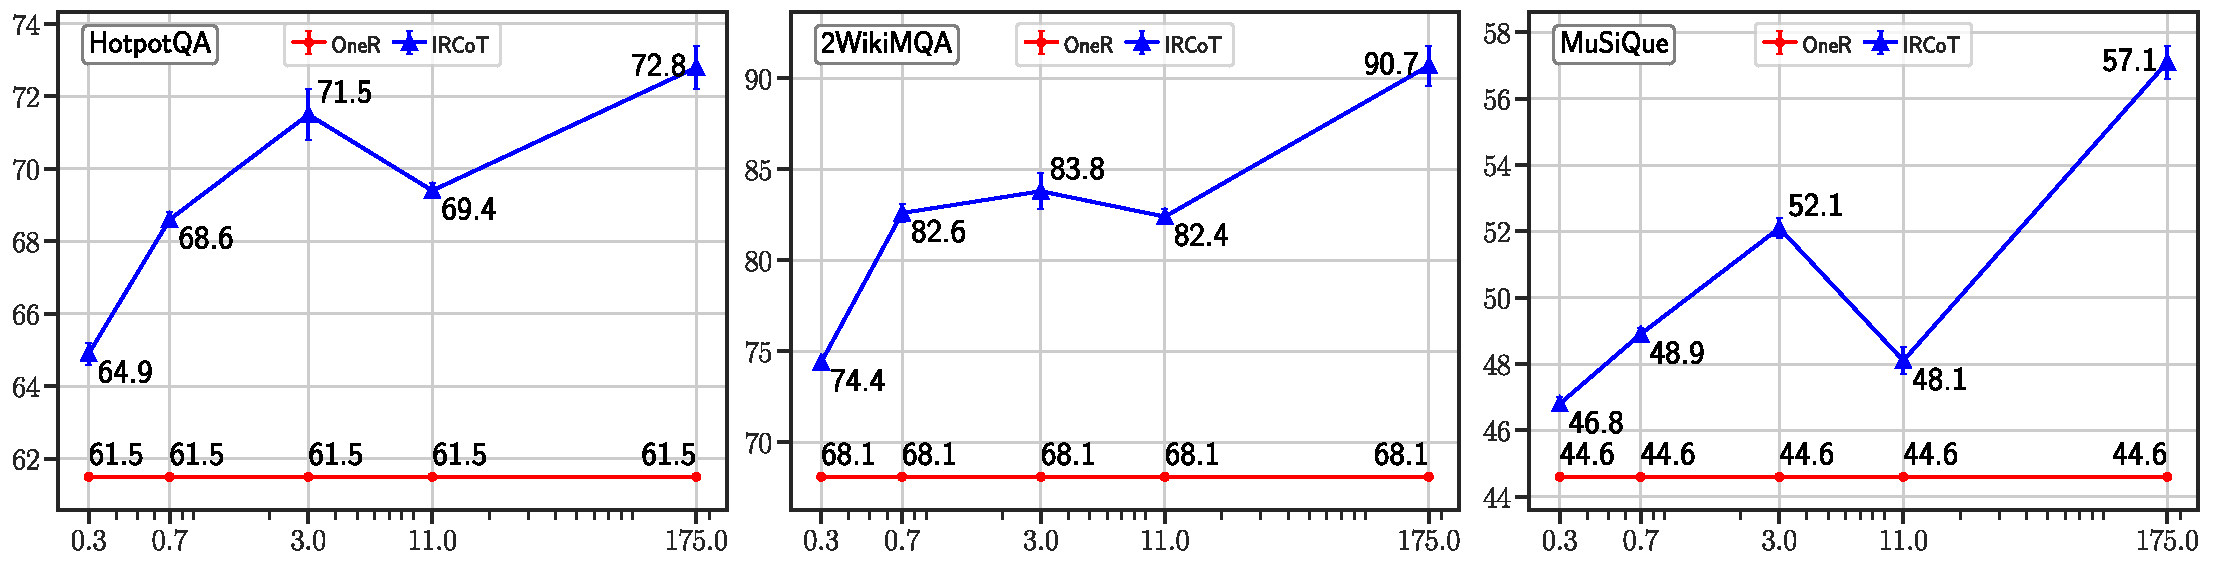
\includegraphics[width=0.95\textwidth]{images/model_scale_retrieval_results.pdf}
\caption{Retrieval recall for OneR (bottom) and \iconsys (top) for LMs of increasing sizes: Flan-T5 \{base (0.2B), large (0.7B), XL (3B), XXL (11B)\} and GPT3 (175B) on HotpotQA, 2WikiMultihopQA, MuSiQue. \iconsys outperforms OneR for all model sizes, including the 0.3B model, and the difference roughly grows with model size. Note: OneR doesn't use LM in its retrieval and so has a fixed score.}
\label{fig:model-scale-retrieval-results}
\end{figure*}

\begin{figure*}[ht]
\centering
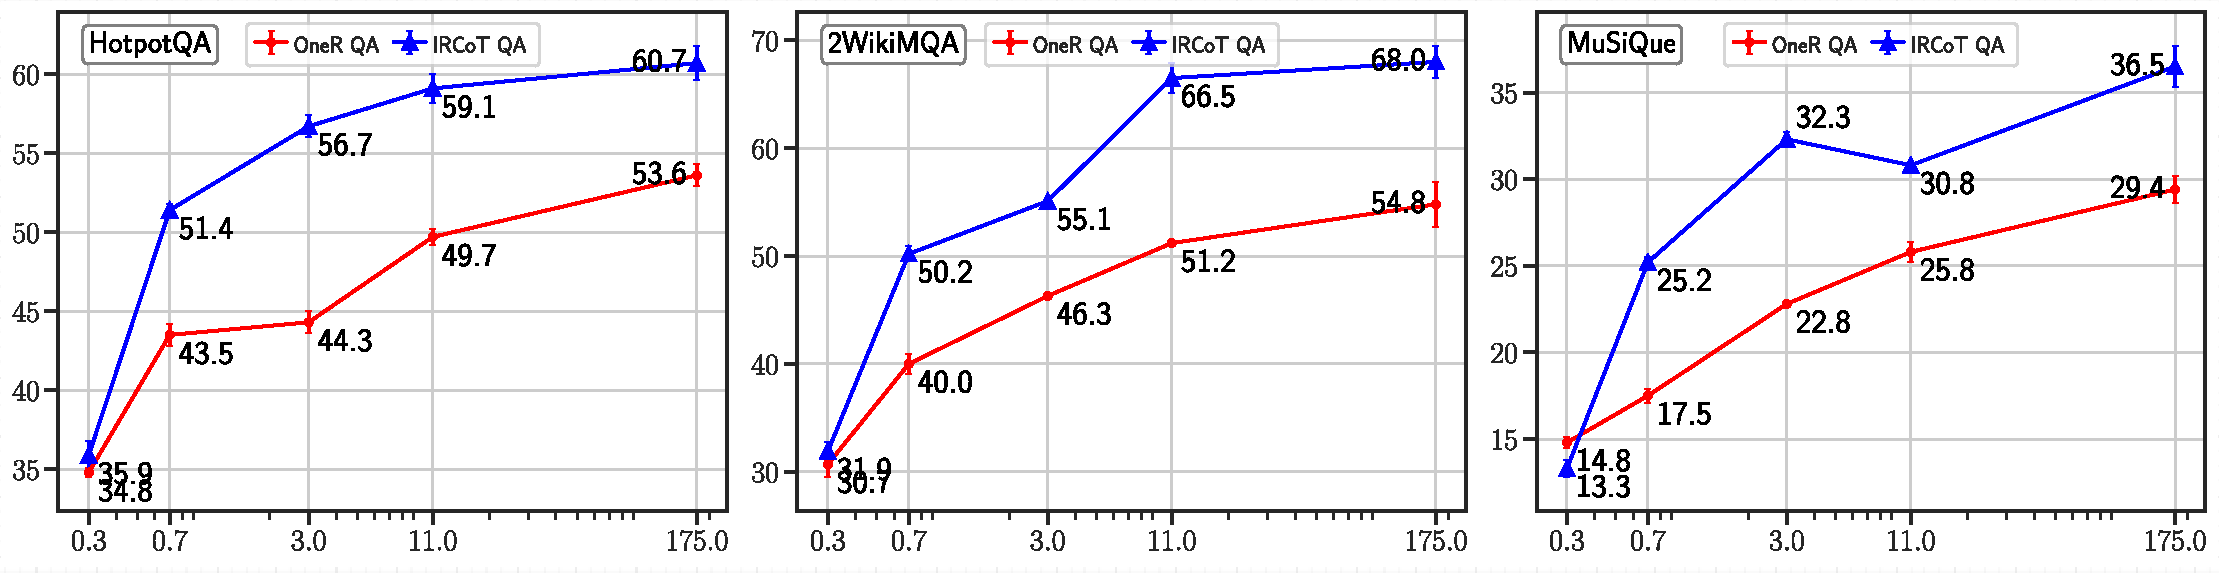
\includegraphics[width=0.95\textwidth]{images/model_scale_qa_results.pdf}
\caption{Answer F1 for ODQA models made using OneR (bottom) and \iconsys (top) for LMs of increasing sizes: Flan-T5 \{base (0.2B), large (0.7B), XL (3B), XXL (11B)\} and GPT3 (175B) on HotpotQA, 2WikiMultihopQA and MuSiQue. \iconsys QA outperforms OneR QA for all model sizes except for the smallest, 0.3B. \iconsys with 3B model even outperforms OneR with 58X larger GPT3 model showing the value of improved retrieval.}
\label{fig:model-scale-qa-results}
\end{figure*}


%%%%%%%%%%%%%%%%%%%%%%%%%%%%%%%%%%%%%%%%%%%%%%%%%%%%
\paragraph{\iconsys is effective in OOD setting. }

Since CoT may not always be easy to write for new datasets, we evaluate NoR, OneR, and IRCoT on generalization to new datasets, i.e. OOD setting. To do so, we use prompt demonstrations from one dataset to evaluate on another dataset.\footnote{We use the evaluation dataset's corpus for retrieval.} For all pairs of the datasets\footnote{We skip IIRC in this exploration as the task is structured a bit differently and requires special handling (see App.~\ref{sec:apndx-iirc-special-handling}).} and for both \texttt{Flan-T5-XXL} and \texttt{GPT3}, we find the same trend as in the IID setting: \iconsys retrieval outperforms OneR (Fig.~\ref{fig:ood-retrieval-results}), and IRCoT QA outperforms both OneR QA and NoR QA (Fig.~\ref{fig:ood-qa-results}).


%%%%%%%%%%%%%%%%%%%%%%%%%%%%%%%%%%%%%%%%%%%%%%%%%%%%
\paragraph{\iconsys generates CoT with fewer factual errors.}

To assess whether our approach also improves the factuality of generated CoTs, we manually annotated CoTs generated by NoR QA, OneR QA, and IRCoT QA using GPT3 for 40 randomly sampled questions from each of the four datasets. We considered CoT to have a factual error if at least one of the facts\footnote{all sentences before the final ``answer is:'' sentence.} is not true.\footnote{Note that factual error doesn't necessarily mean the predicted answer is incorrect and vice-versa. This is because the model can generate a wrong answer despite all correct facts, and vice-versa. We also account for the possibility of answer annotation errors in the original datasets.} As Fig.~\ref{fig:cot-factual-errors} shows, NoR makes the most factual errors, OneR makes fewer, and \iconsys the least. In particular, \iconsys reduces the factual errors over OneR by 50\% on HotpotQA and 40\% on 2WikiMultihopQA.


Table~\ref{table:nor-oner-cot-examples} illustrates how the CoT predictions for different methods vary qualitatively. Since NoR relies completely on parametric knowledge, it often makes a factual error in the first sentence, which derails the full CoT. OneR can retrieve relevant information closest to the question and is less likely to make such errors early on, but it still makes errors later in the CoT. IRCoT, on the other hand, is often able to prevent such errors in each step.

%%%%%%%%%%%%%%%%%%%%%%%%%%%%%%%%%%%%%%%%%%%%%%%%%%%%
\paragraph{\iconsys is also effective for smaller models.}

To see how effective \iconsys is at different LM sizes, we show the scaling plots in Fig.~\ref{fig:model-scale-retrieval-results}.\footnote{We skip IIRC here as the smaller models are not good at identifying Wikipedia titles from a paragraph and a question which is necessary for IIRC (see App.~\ref{sec:apndx-iirc-special-handling}).} We compare the recall for OneR and \iconsys using \texttt{Flan-T5} \{base (0.2B), large (0.7B), XL (3B), XXL (11B)\}, and GPT3 \texttt{code-davinci-002} (175B). \iconsys with even the smallest model (0.2B) is better than OneR, and the performance roughly improves with the model size. This shows the CoT generation capabilities of even small models can be leveraged for improving retrieval. Furthermore, we show the effect of model size on the QA score in Fig.~\ref{fig:model-scale-qa-results}. For all sizes except the smallest (0.2B), we see \iconsys QA is better than OneR QA. Moreover, \iconsys with a 3B model even outperforms OneR and NoR with a 58X larger 175B GPT3 model in all datasets.


%%%%%%%%%%%%%%%%%%%%%%%%%%%%%%%%%%%%%%%%%%%%%%%%%%%%
\paragraph{\iconsys is SOTA for few-shot multistep ODQA.\footnote{\label{footnote:sota}App.~\S\ref{sec:sota-differences} reports updated SOTA numbers, including contemporaneous and newer works.}}


We compare \iconsys QA with five recent approaches to using LLMs for ODQA: Internet-Augmented QA~\cite{internet-augmented-qa}, RECITE~\cite{recitationlm} ReAct~\cite{react}, SelfAsk~\cite{selfask}, and DecomP~\cite{old-decomp}. Although these are not head-to-head comparisons as different methods use different APIs, knowledge sources, and even LLMs (see App.~\ref{sec:sota-differences} for details), it is still informative to explore, in a leaderboard-style fashion, how \iconsys performs relative to the best numbers published for these recent systems.

\vspace{0.1cm}
\begin{table}[ht]
    \centering
    \footnotesize
    \setlength{\tabcolsep}{2.0pt}
    \begin{tabular}{ccccc}\toprule
        Model &  HpQA\textsuperscript{Br}  &  HpQA & 2WikiMQA & MQ\textsuperscript{2H} \\
        \midrule
        InterAug      &   $-$ | $-$    &        30.3 | $-$\p{xx}   &        $-$ | $-$        &        $-$ | $-$            \\
        RECITE        &   $-$ | $-$    &        37.1 | 48.4        &        $-$ | $-$        &        $-$ | $-$            \\
        ReAct         &   $-$ | $-$    &        35.1 | $-$\p{xx}   &        $-$ | $-$        &        $-$ | $-$            \\
        SelfAsk       &   $-$ | $-$    &         $-$ | $-$         &       40.1 | $-$\p{xx}   &       15.2 | $-$\p{xx}     \\
        DecomP        &  \p{x..}$-$ | 50.0  &         $-$ | $-$         &   \p{x..}$-$ | 59.3      &       $-$ | $-$       \\
        \midrule
        \sys QA       &   \textbf{45.8 | 58.5}   &    \bf{49.3 | 60.7}       &   \bf{57.7 | 68.0}      &  \bf{34.2 | 43.8} \\
        \bottomrule
    \end{tabular}
    \caption{Comparison with other LLM-based ODQA systems on EM and F1 scores. `$-$': score is unavailable. HpQA\textsuperscript{Br}: Bridge questions subset of HotpotQA. MQ\textsuperscript{2H}: MuSiQue 2-hop questions. \iconsys QA with GPT3 (ours) outperforms other systems by a large margin. Note: Comparisons aren't head-to-head as discussed in the text. App.~\S\ref{sec:sota-differences} reports updated SOTA numbers, including contemporaneous and newer works.
    \label{table:extrinsic-comparison}
    }
\end{table}


As shown in Table~\ref{table:extrinsic-comparison}, \iconsys QA significantly outperforms all of these recent systems by a large margin, setting a new state of the art in terms of what's achievable via retrieval-augmented LLMs (without supervised training).



\begin{table*}[t]
    \centering
    \footnotesize
    \setlength{\tabcolsep}{4.0pt}
    \begin{tabular}{llllll}\toprule
        & \textbf{Question} &   \textbf{Gold Facts} & \textbf{NoR QA} & \textbf{OneR QA} & \textbf{IRCoT QA} \\
        \midrule

        % HotpotQA
        \multirow{2}{*}{\rotatebox[origin=c]{90}{\parbox[c]{3.0cm}{\centering HotpotQA}}}
        & \begin{minipage}[t]{2cm} The tap dancing soloist in My Feet Keep Dancing also starred in what 1935 MGM musical? \end{minipage}
        & \begin{minipage}[t]{3.0cm} $\Rightarrow$ The tap dancing soloist in My Feet Keep Dancing is \textcolor{blue}{Fayard Nicholas}. \\ $\Rightarrow$ Fayard Nicholas starred in the 1935 MGM musical \textcolor{blue}{An All-Colored Vaudeville Show}. \end{minipage}
        & \begin{minipage}[t]{3.0cm} The tap dancing soloist in My Feet Keep Dancing is \textcolor{red}{Eleanor Powell}. Eleanor Powell also starred in the 1935 MGM musical \textcolor{red}{Broadway Melody} of 1936. So the answer is: Broadway Melody of 1936. \end{minipage}
        & \begin{minipage}[t]{3.0cm} The tap dancing soloist in My Feet Keep Dancing is \textcolor{blue}{Fayard Nicholas}. Fayard Nicholas also starred in the 1935 MGM musical \textcolor{red}{Top Hat}. So the answer is: Top Hat. \end{minipage}
        & \begin{minipage}[t]{3.0cm} The tap dancing soloist in My Feet Keep Dancing is \textcolor{blue}{Fayard Nicholas}. Fayard Nicholas starred in the 1935 MGM musical \textcolor{blue}{An All-Colored Vaudeville Show}. So the answer is: An All-Colored Vaudeville Show. \end{minipage} \\

        \midrule

        % 2WikiMultihopQA
        \multirow{1}{*}{\rotatebox[origin=c]{90}{\parbox[c]{4.0cm}{\centering 2WikiMQA}}}
        & \begin{minipage}[t]{2cm} Who is the father-in-law of Queen Hyojeong? \end{minipage}
        & \begin{minipage}[t]{3.0cm} $\Rightarrow$ Queen Hyojeong is the wife of \textcolor{blue}{King Heonjong of Joseon}. \\ $\Rightarrow$ King Heonjong of Joseon is the son of \textcolor{blue}{Crown Prince Hyomyeong}. \end{minipage}
        & \begin{minipage}[t]{3.0cm} Queen Hyojeong has a husband named \textcolor{red}{King Gojong}. King Gojong has a father named \textcolor{red}{Heungseon Daewongun}. Thus, Queen Hyojeong has a father-in-law named Heungseon Daewongun. So the answer is: Heungseon Daewongun. \end{minipage}
        & \begin{minipage}[t]{3.0cm} Queen Hyojeong is the wife of \textcolor{blue}{King Heonjong of Joseon}. King Heonjong of Joseon is the son of \textcolor{red}{King Sejo of Joseon}. Thus, King Sejo of Joseon is the father-in-law of Queen Hyojeong. So the answer is: King Sejo of Joseon. \end{minipage}
        & \begin{minipage}[t]{3.0cm} Queen Hyojeong is the wife of \textcolor{blue}{King Heonjong of Joseon}. King Heonjong of Joseon is the son of \textcolor{blue}{Crown Prince Hyomyeong}. Thus, Crown Prince Hyomyeong is the father-in-law of Queen Hyojeong. So the answer is: Crown Prince Hyomyeong. \end{minipage} \\

        \midrule

        % MuSiQue
        \multirow{1}{*}{\rotatebox[origin=c]{90}{\parbox[c]{3.0cm}{\centering MuSiQue}}}
        & \begin{minipage}[t]{2cm} What is the name of the castle in the city where the performer of A Collection 1984–1989 was born? \end{minipage}
        & \begin{minipage}[t]{3.0cm} $\Rightarrow$ A Collection 1984–1989 was performed by \textcolor{blue}{Jane Siberry}. \\ $\Rightarrow$ Jane Siberry was born in \textcolor{blue}{Toronto}. \\ $\Rightarrow$ The castle in Toronto is the \textcolor{blue}{Casa Loma}. \end{minipage}
        & \begin{minipage}[t]{3.0cm} The performer of A Collection 1984–1989 is \textcolor{red}{The The}. The The was born in \textcolor{red}{London}. The name of the castle in London is the \textcolor{red}{Tower of London}. So the answer is: the Tower of London. \end{minipage}
        & \begin{minipage}[t]{3.0cm} A Collection 1984–1989 was performed by \textcolor{blue}{Jane Siberry}. Jane Siberry was born in \textcolor{blue}{Toronto}. The castle in Toronto is \textcolor{red}{Peqin Castle}. So the answer is: Peqin Castle. \end{minipage}
        & \begin{minipage}[t]{3.0cm} A Collection 1984–1989 was performed by \textcolor{blue}{Jane Siberry}. Jane Siberry was born in \textcolor{blue}{Toronto}. The castle in Toronto is the \textcolor{blue}{Casa Loma}. So the answer is: Casa Loma. \end{minipage} \\

        \bottomrule

    \end{tabular}
    \caption{Example CoTs generated by GPT3 with different methods. Since NoR relies on parametric knowledge, it often makes a factual error in the first sentence derailing the full CoT. OneR can retrieve relevant information closest to the question and is less likely to make such errors early on, but it still makes errors later in the CoT. As \iconsys performs retrieval after each step, it is often able to prevent such errors in each step. More examples are in App.~\ref{sec:apdx-nor-oner-cot-examples}.}
    \label{table:nor-oner-cot-examples}
\end{table*}







